\chapter{Resultados e Discussões}	

A caracterização do arcabouço estrutural utilizando métodos sismológicos possui problemas de unicidade de solução, como outros métodos geofísicos.  Essa falta de informação direta do objeto em estudo proporciona uma gama de soluções. Porém há inúmeros meios de se contornar tal situação. A modelagem mostra se a técnica tem resolução para seu objetivo.

Para delimitar as principais feições utilizou-se de modelos simples, como visto na Figura \ref{modelagem}-a, apenas com camadas planas, com esses modelos pode-se mostrar que as estimativas da espessura crustal e são consistentes com os dados observados. Na modelagem utilizou-se os programas "\textit{icmod}", "\textit{icmod}", "\textit{vplot[s]}", "\textit{respknt}",  e "\textit{pwaveqn}", disponibilizados por \cite{Ammon_waterlevel_1997}.

\begin{figure}[!ht]
\centering
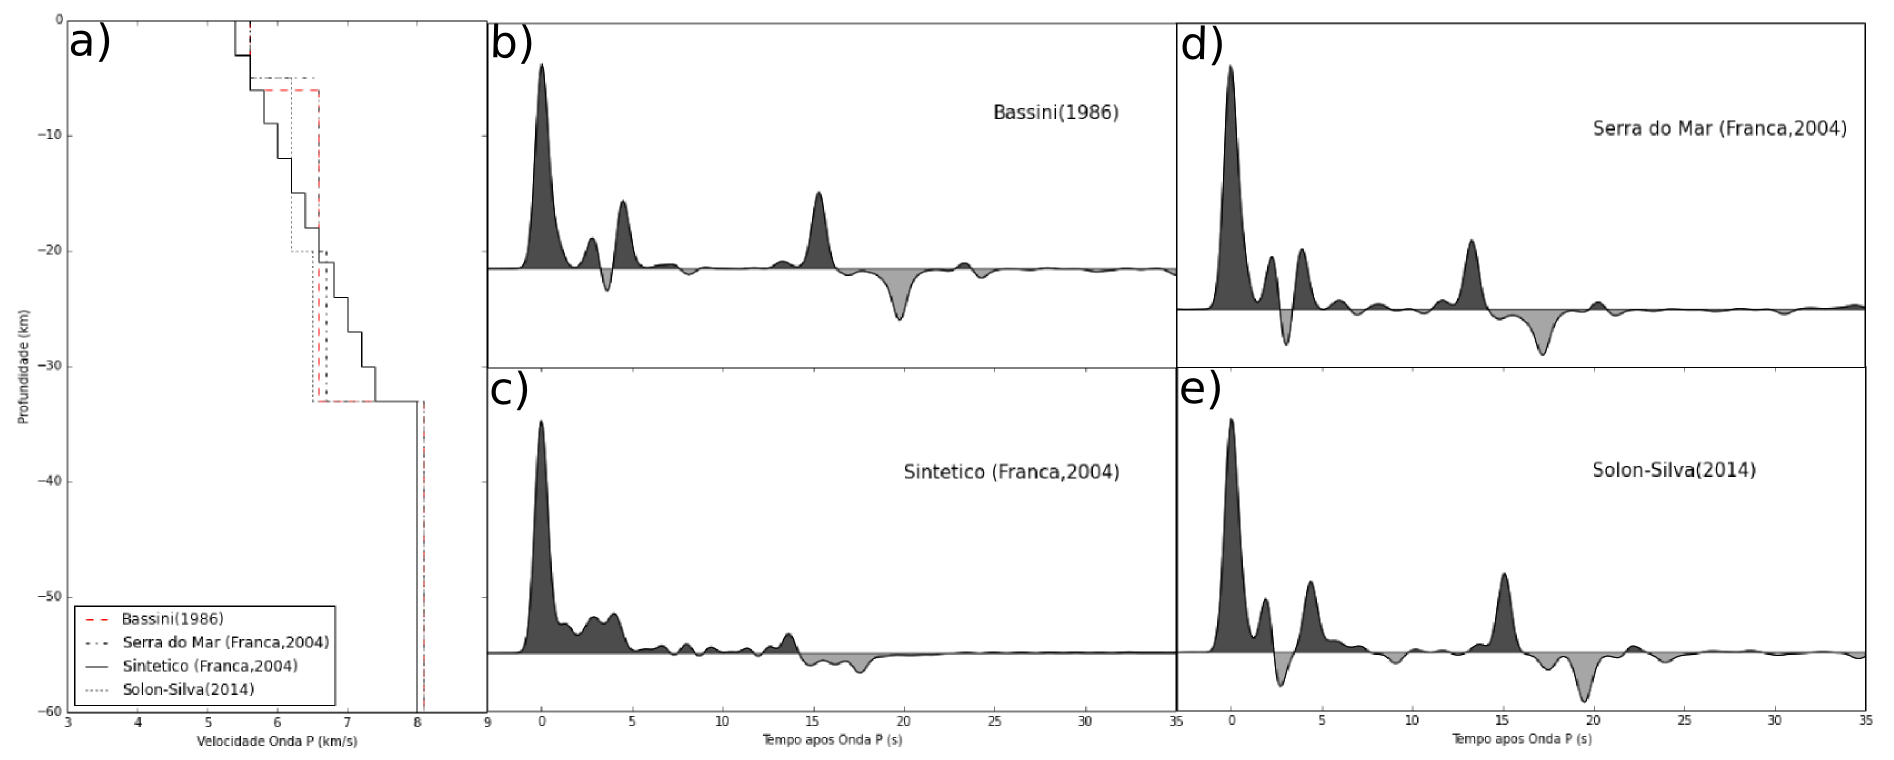
\includegraphics[scale=0.5]{modelagem_RF.png}
\caption{}
\label{modelagem}
\end{figure}

Figure \ref{RF_perfil} shows a section of Receiver Functions obtained from several events come from the northwest region and normalized by the amplitude of the first peak. The first peak is the direct P-wave arrival, the second highest, around 5 seconds, is the P wave converted to S wave at the Moho discontinuity.


The multiples PpPs and PpSs+PsPs have much lower amplitude than the P-to-S conversion. We noted in Figure \ref{RF_perfil} that the Moho depth estimated higher in the inner of the continent than the coast. We also identified signals before the Moho, around 2 to 4 seconds, which vary along the profile. This can be related to interfaces with a relatively high contrast of physical property. The negative pulse may indicate the existence of a low-velocity layer. According with geological setting, we can infer that layer is the Taubat\'{e} basin, because this basin is located in a rift system, in the dark area in the Figure \ref{Map_loc}.The solutions found corroborate with the results from \cite{assumpcao_models_2013}, \cite{assumpcao_crustal_2013} and \cite{van_der_meijde_gravity_2013}  using data from compilations of works in South America and Brazil. The uncertainties of data are linked to the quality and the quantity of the Receiver Functions. The estimated values of the Moho depth for each station were linearly interpolated to generate a regional map, shown in Figure. In order to improve the interpolation, we added data from \citep{assumpcao_crustal_2013}. In Figure \ref{figura7}, we can see the Moho thinning in direction to the east.


The Figure \ref{figura3} shows the registered events in STA08 station. The most part of seisms recorded in stations are events from Andes range or Central America.

 
The results from the Figure \ref{figura4} allows a fast evaluation of the data quality. We observed some curves diverging with the superior and inferior bounds of noise, but are punctual events with a low probability (violet curves). In majority of stations the curves were found in the intermediary zone, shown a data quality good to moderate.



In some stations, high probabilities appear in short and long period. This is related with diurnal variations. These changes are connected with human activity (short period) and temperature (long period). In general, the noise of short period is compound for noise generated in humans activities, with interval between 1 and 15 seconds, as shown in Figure \ref{figura4}. This noise type is dominated for micro-seisms. In noise of long period ($>$30 s) the influence of atmospheric pressure variation and temperature can alter the noise level. In case of temporary installation, the thermic isolation is basic, which carries a high level of long period noise. The quakes generate signal of high frequency (1-10 Hz), in case of local or regional seisms, already the teleseisms are of long period (10-20 seconds).

The Figure \ref{figura5} shows a section of Receiver Functions obtained from several events and normalized by the amplitude of the first peak. The first peak is the direct P-wave arrival, the second highest, around 5 seconds, is the P wave converted to S wave in the Moho discontinuity. 



The multiples PpPs e PpSs+PsPs not have a high amplitude. The Figure \ref{figura5} shows also the deconvolution of transversal component by the vertical component.Assuming a medium, without lateral variation, the deconvolution should be zero. The small amplitude of transversal component suggests a little lateral alteration in the properties of medium. To amplify the signal-noise ratio of second peak in Receiver Functions a simple stacking of all functions was realized. After, the data separation in four groups divided by the azimuth between the quake and the station. 

We noted in Figure \ref{figura6} a substantial subsidence under the station STA04. We realized signals before the Moho, among 2 and 4 seconds, who have a depth variations along the profile. This can be related to interfaces with a contrast of different physical property. The negative pulse, red color, indicates an existence of a low-velocity layer. According with geological setting, we can infer that layer is the Taubat\`{e} basin, because this basin is located in a rift system, and this explain the subsidence of Mantle.

We calculated the crustal thickness (H) that maximizes the value of real amplitudes of Receiver Function. The best combination of crustal thickness and $v_{p}/v_{s}$ ratio calculated for each station is found in Table \ref{tabela}. The solutions found corroborate with the results from \cite{assumpcao_models_2013}, \cite{assumpcao_crustal_2013} and \cite{van_der_meijde_gravity_2013} in data of compilations from works of South America and Brazil. The obtained values for crustal thickness in Table \ref{tabela} are according with the mean measured by \cite{assumpcao_models_2013}, \cite{assumpcao_crustal_2013} and \cite{van_der_meijde_gravity_2013}, is about 30~40 km.


The uncertainty, shown in Table \ref{tabela} are linked to quality and quantity of the Receiver Functions. A important phase is the selection of the best Receiver Functions, because the data quality is preponderant over the quantity. The uncertainty associated a each one of obtained parameters by the method Hk and estimated generally by "bootstrap" method, developed for  \citep{efron_statistical_1991}. From the original set of Receiver Functions the program generates subsets containing traces randomly selected. These method is repeated for each subsets, resulting in a parameter set H and $v_{p}/v_{s}$ .Mean and standard deviation from the values provide us a mean value and an estimate of the uncertainty associated to determination. There is no rule for determining the number subsets that must be generated, the crucial is search a value that makes the estimative stabilize,  including uncertainties. In general we use a value between 100 and 200 subsets depending on the amount de traces available during the “bootstrap”.

The calculated values of the Moho depth for each station were linearly interpolated to generate a regional map, shown in the Figure \ref{figura7}. To improve the interpolation, we added data from \citep{assumpcao_crustal_2013}. In the Figure \ref{figura7} we can see the Moho thinning in direction to east, reinforcing the proximity with the oceanic crust.

